\documentclass{article}
\usepackage[margin=1in]{geometry}
\usepackage{amsmath,amsthm,amssymb}
\usepackage{bbm,enumerate,mathtools}
\usepackage{tikz,pgfplots}
\usepackage{chessboard}
\usepackage[hidelinks]{hyperref}
\usepackage{multicol} % Problem 35

\newenvironment{question}{\begin{trivlist}\item[\textbf{Question.}]}{\end{trivlist}}
\newenvironment{note}{\begin{trivlist}\item[\textbf{Note.}]}{\end{trivlist}}
\newenvironment{references}{\begin{trivlist}\item[\textbf{References.}]}{\end{trivlist}}
\newenvironment{related}{\begin{trivlist}\item[\textbf{Related.}]\end{trivlist}\begin{enumerate}}{\end{enumerate}}


\begin{document}

\rating{1}{1}
Suppose that you're on an $n \times m$ grid, and you'd like to place rectangles
to fill up as many gridlines as possible---the catch is that if there are an
even  number of boxes on a gridline, then they cancel out.

\begin{figure}[ht!]
  \centering
  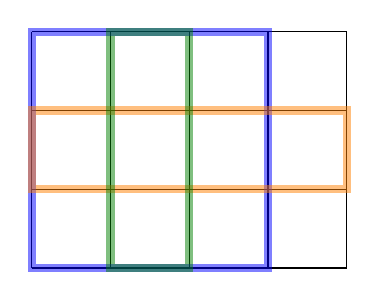
\begin{tikzpicture}
    \draw (0,0) grid (4, 3);
    \draw[line width=3, blue, opacity=0.5] (0,0) rectangle (3,3);
    \draw[line width=3, orange, opacity=0.5] (0,1) rectangle (4,2);
    \draw[line width=3, green!50!black, opacity=0.5] (1,0) rectangle (2,3);
  \end{tikzpicture} ~~
  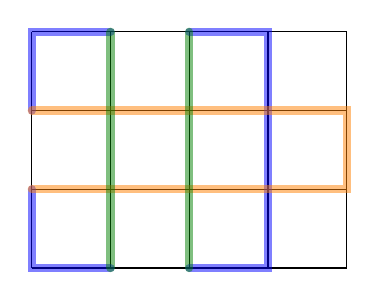
\begin{tikzpicture}
    \draw (0,0) grid (4, 3);
    \draw[line width=3, blue, opacity=0.5, line cap=round]
      (0,1)--(0,0)--(1,0)
      (2,0)--(3,0)--(3,3)--(2,3)
      (1,3)--(0,3)--(0,2);
    \draw[line width=3, orange, opacity=0.5, line cap=round]
      (0,1)--(4,1)--(4,2)--(0,2);
    \draw[line width=3, green!50!black, opacity=0.5, line cap=round]
      (1,0)--(1,3)
      (2,0)--(2,3);
  \end{tikzpicture}
  \caption{This arrangment with three boxes on the $4 \times 3$ grid misses
  only seven edges.}
\end{figure}

\begin{question}
  What is the greatest number of edges that can be covered?
\end{question}

\begin{related}
  \item How many minimal arrangments of rectangles are there? (Right example)
  \item How many maximal edge covers are there? (Left example)
  \item What if the rectangles must be square?
  \item What if a maximum of $k$ rectangles is allowed?
  \item What if it takes 3 (or $c$) rectangles to cancel out?
  \item Is this equivalent to finding disjoint collections of ``almost''
    Eulerian cycles on a grid graph?
  \item How does this generalize to higher dimensions, the triangular grid, etc?
  \item What if we want to cover vertices instead of edges? Facets?
  \item How many edges are covered if we use every possible rectangle?
  \item Placement of rectangles generates an abelian group.
    What is the group's structure?
    Is the size of the group the number of possible edge covers?
\end{related}

\begin{references}
  \item \url{https://math.stackexchange.com/q/1579862/121988}
  \item Problems 37 and 74.
\end{references}
\end{document}
